% We propose an optimized snapshot program to locate the first ever
% multiply-imaged supernova. This program is now feasible on HST thanks
% to the dozens of galaxy clusters that now have deep WFC3-IR imaging
% and well-modeled lens models.  Facilitated by the accompanying small
% GO followup program (PI: Strolger), this unprecedented discovery will
% set the stage for the first ever use of a supernova for time delay
% cosmography, providing a measure of $H_0$ to
% within 10\% precision {\em without reference to the local distance
% ladder}. This first supernova time delay will deliver a valuable test
% of systematic biases in other cosmological probes, and will serve as a
% pathfinder for future samples of lensed supernovae with JWST and LSST.
%
%\medskip

% \noindent {\bf Motivation~~~}

Exactly fifty years ago, \citet{Refsdal:1964} first imagined the use
of multiply-imaged supernovae (SNe) to measure the Hubble
constant, \Ho, through time delay cosmography (see inset, below).
Over the intervening 5 decades, no multiply-imaged SN has been found.
With this program we propose to use a WFC3-IR snapshot survey of
strong lensing galaxy clusters, providing the first truly viable
opportunity to find a multiply-imaged SN.  This project is newly
possible with HST because we can now capitalize on a treasury
of well-studied strong lensing clusters with deep WFC3-IR template
imaging.  This provides the critical advantage that we can detect SN
at $z\sim2$ where we have a large sample of known multiply-imaged
galaxies in an era when the universe was near peak efficiency for
generating SN explosions.

\bigskip

\noindent {\bf The First Multiply Imaged SN:~~~}
After several decades of substantial effort and slow progress, the
time delay field is now rapidly maturing \citep[see][for recent
reviews]{Jackson:2007,Treu:2010}. There already exists a sample of
$\sim$20 time delay measurements for multiply-imaged \emph{quasars},
which are typically lensed by a single foreground galaxy, with only a
\begin{wrapfigure}{r}{0.65\textwidth}
\vspace{-1em}
\framebox{
\begin{minipage}{0.64\textwidth}
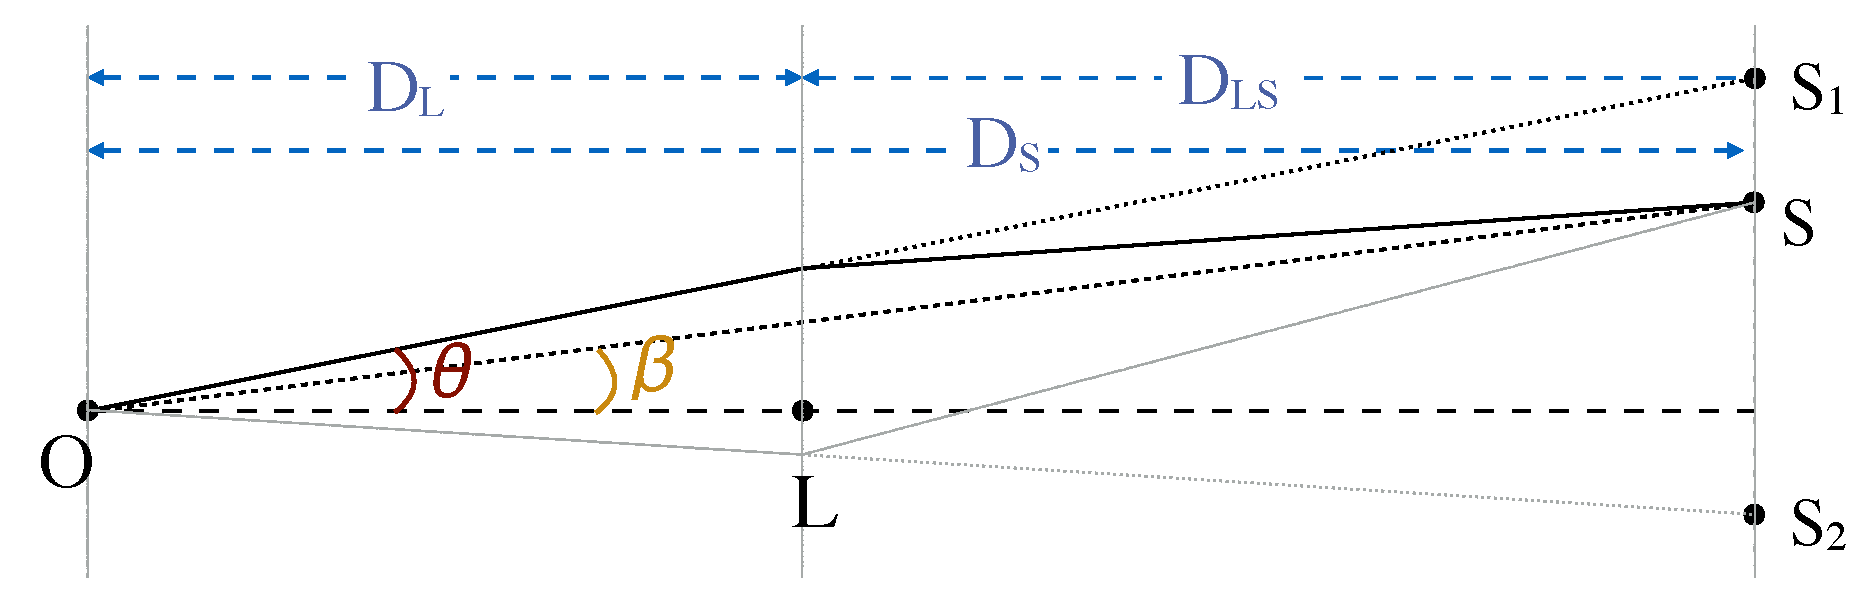
\includegraphics[width=0.9\textwidth]{FIG/lensingGeometry2}
\begin{small}
{\bf Time Delay Cosmography: }  
As light from a distant
source passes through a gravitational lens, each subsequent image will
appear to the observer delayed by 
\begin{equation}\label{eq:dt}
  \dt = \frac{(1+z_L)}{c}\frac{\Dl \Ds}{\,\Dls} \left(\frac{1}{2}(\theta-\beta)^2 - \psi(\theta)\right)
\end{equation}
\noindent (relative to the unlensed travel time). Here, $z_L$ is the redshift of the lens, while \Dl, \Ds, 
and \Dls\ are angular diamater distances from the observer to the
lens, observer to source, and lens to source, respectively.  The time
delay has a geometric component due to light rays following different
path lengths to the observer, plus a general relativistic component,
$\psi$, due to differing values of the gravitational potential along
each path. The distance ratio $\Dl\Ds/\Dls$ in Eq.~\ref{eq:dt} carries
a factor \Ho$^{-1}$, so if the lensing potential $\psi$ is well known,
then the {\bf \em time delay measurement  provides a direct constraint on
the Hubble constant that is completely independent of the local distance
ladder.}
\end{small}
\end{minipage}}
\end{wrapfigure}
few that are known to be lensed by galaxy
clusters \citep{Inada:2003,Inada:2006,Oguri:2008,Dahle:2013}.  As
techniques for measuring the time delay \dt\ and modeling the lensing
potential $\psi$ have improved, there are now a few of these lensed
quasars that can jointly deliver an \Ho\ constraint with $\sim$6\%
precision \citep[e.g.][]{Suyu:2010,Suyu:2013}.  Additionally, time
delay distances provide an especially powerful check for unknown
systematics, because each separate time delay measurement can be
individually quite precise and largely independent of the rest of the
sample \citep{Suyu:2013,Treu:2013}.

A measured time delay from even a single multiply-imaged SN would be a
valuable addition, and would provide a critical first step towards
future samples with over 100 SN time delays in the JWST/LSST
era. Additionally, if the lensed SN is of Type Ia (a likely prospect
for our survey strategy), then light curve fitting can provide a
luminosity distance measurement with $\sim$8\%
precision \citep[e.g.][]{Phillips:1993,Jha:2007}. With a known
luminosity distance, the source magnification can be directly
measured, providing powerful additional leverage for breaking
degeneracies in the lens
model \citep{Kolatt:1998,Oguri:2003}. Finally, a lensed SN discovered
with this program could easily be among the most distant SNe ever
seen, very valuable in its own right.


% \bigskip

\medskip
\noindent {\bf How many SNAPs?~~~}
To estimate the number of snapshots we need, we start with an
optimized list of target clusters (Table~\ref{tab:clusters}).  We then
tabulate all the known multiply-imaged galaxies behind those clusters.
These are our potential SN host galaxies, and we count each separate
image of a multiple-image set except the last one (one cannot measure
a time delay from the last appearance).  The time delay between each
image is of order months or years, so each snapshot visit is
essentially observing the same galaxy at several widely-spaced epochs
that can be treated as independent.  We then limit this list to count
only those image pairs that would have a time delay of \dt$<$5 years
leaving us with an average of $\sim15$
potential lensed SN host galaxies per cluster.\footnote{Note that this
computation of the SN yield by counting known galaxies is a relatively
conservative approach.  It is quite possible to detect a
multiply-imaged SN even if the host galaxy remains undetected. Such
apparently ``hostless'' SN could boost our actual probability of a
successful detection by as much as $\sim$20\%.}

For each lensed galaxy, we can then compute the total number of
detectable core collapse (CC) and Type Ia SN (\SNIa) per snapshot as

\begin{equation}\label{eq:SNR}
N_{\mbox{det}} = (SNR_{Ia} \cdot t_{vis,Ia} + SNR_{CC} \cdot t_{vis,CC})  (1+z)^{-1},
\end{equation}

\noindent where SNR is the SN explosion rate
per year (separately computed for each galaxy and segregated by SN
type), $t_{vis}$ is the fraction of a year that an average SN is brighter
than our snapshot detection limits (see
Table~\ref{tab:detectionLimits}, below), and the factor of $(1+z)^{-1}$
corrects for time dilation at the redshift of the galaxy.
Using simulated SN light curves in 240 multiply-imaged
galaxies (Figure~\ref{fig:tvis}), we find an average $t_{vis}\sim 30$
days for \SNIa\ and $\sim$20 days for SN II.

To estimate SNR$_{Ia}$, we start with the volumetric SN rate as a
function of redshift, SNR$_{Vol}$, as measured out to $z\sim2.5$
\citep{Graur:2014,Rodney:2014}.  Dividing by the measured
cosmic luminosity density \citep{Reddy:2009}, we convert this volumetric
rate to a SN rate per unit B-band luminosity SNR$_{B}$.  We then multiply by
the observed luminosity of each galaxy to get SNR$_{Ia}$ for
Eq.~\ref{eq:SNR}.

For core collapse SN, which are even more tightly correlated to star
formation than are \SNIa, we use the observed rest-frame UV luminosity
to define each galaxy's star formation rate, using 
$SFR = 9.3\times 10^{-29} \cdot L_{UV}$ \Msun yr$^{-1}$ \citep{Dahlen:2007}, and
then convert to SN rate using $SNR_{CC} = 0.007 \cdot SFR$, as appropriate
for a Schechter luminosity function and consistent with
observations \citep{Dahlen:2012}.  

Folding in these values for all multiply-imaged galaxies in a
representative sample from our target list of clusters, we find
$N_{det}=0.01$ SN discoveries per snapshot observation.\footnote{Note
that this predicted yield is unchanged if we instead use observed SN
rates from the local universe \citep[e.g.][]{Mannucci:2005,Li:2011b},
appropriately scaled to account for the increased star formation at
$z\sim2$}. This means that we need only $\sim$100 executed snapshots
to have a good chance at catching the first ever multiply imaged
SN. Factoring in an anticipated execution fraction of $\sim$30\%, we
request 300 snapshots to deliver this valuable cosmographic tool.






